\documentclass{article}

\usepackage{graphicx}
\usepackage{tikz}
\usepackage{tikzsymbols}
\usetikzlibrary{calc,patterns,shapes.geometric}
\pagestyle{empty}
\usepackage[margin=0pt]{geometry}
\geometry{papersize={14in,12in}}

\def\centerarc[#1](#2)(#3:#4:#5){\draw[#1] ($(#2)+({#5*cos(#3)},{#5*sin(#3)})$) arc (#3:#4:#5);}

\begin{document}
	\begin{figure}
		\centering
		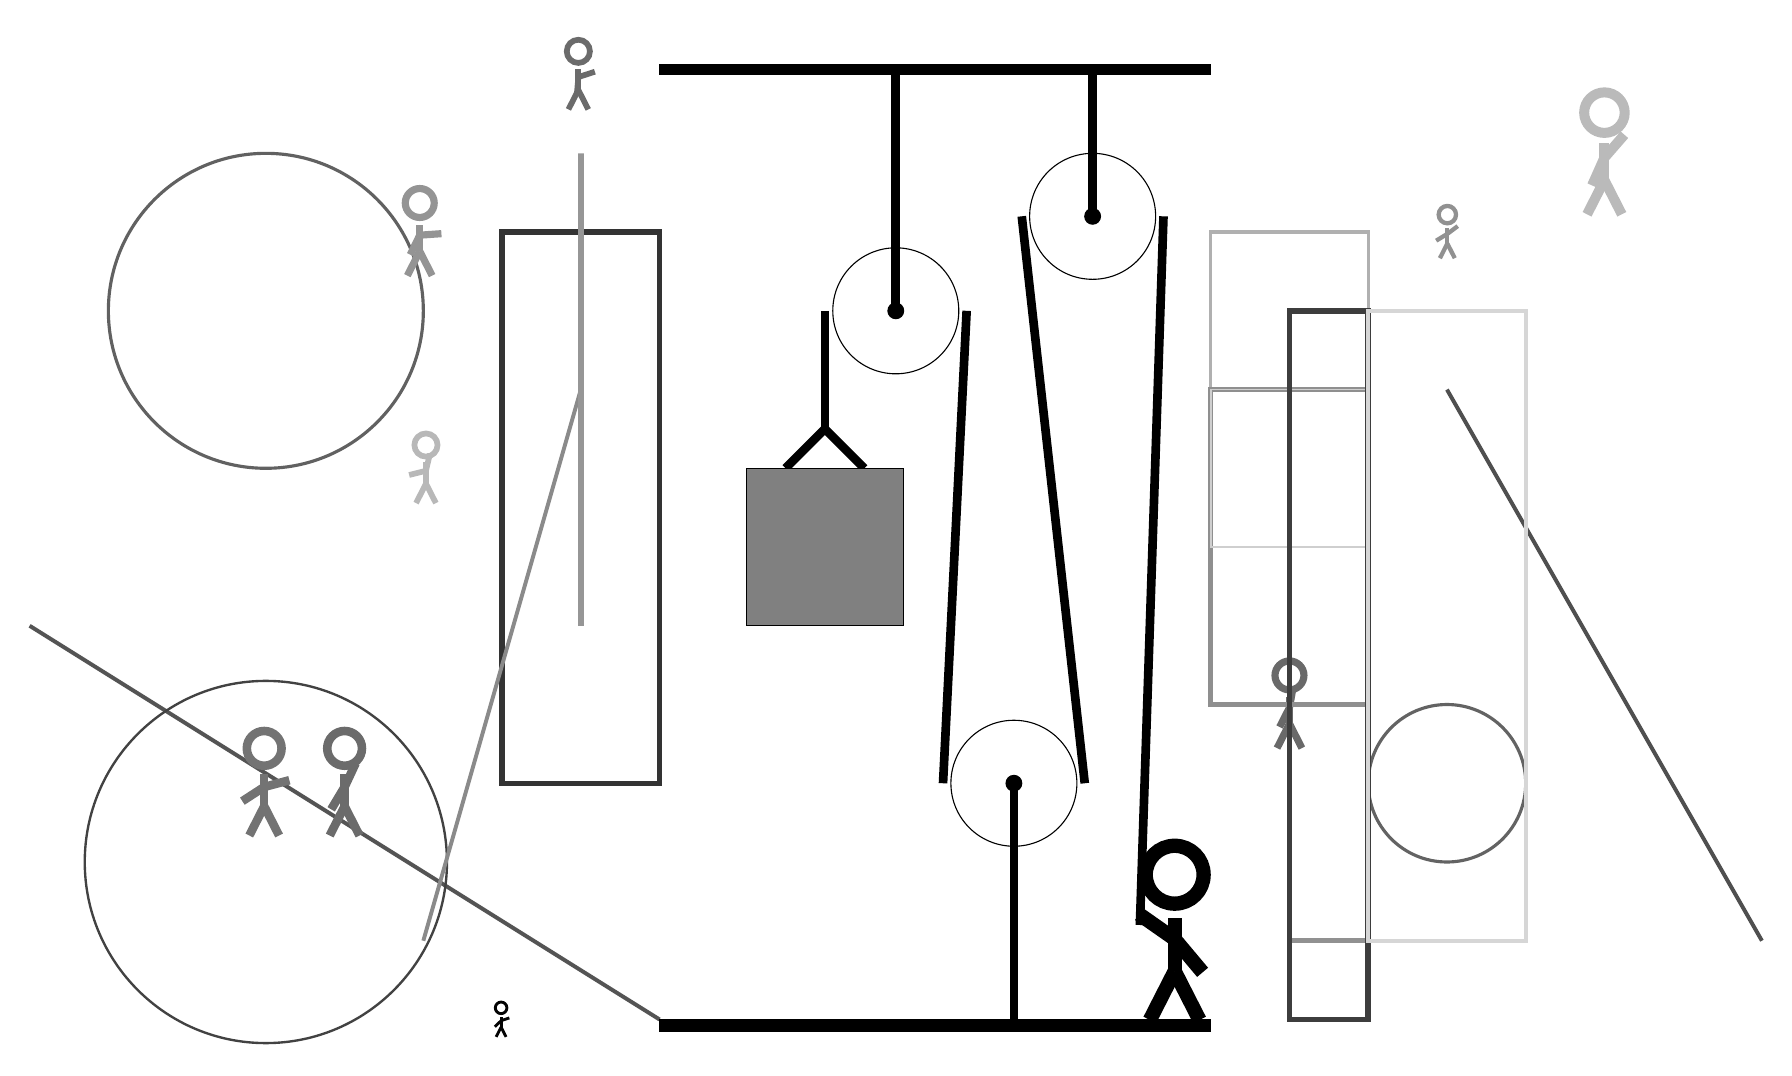
\begin{tikzpicture}
			%%%%% START %%%%%
			
			\draw[fill=black] (-2, 9) rectangle (5, 9.125);
			
			\draw (1, 6) circle (0.8);
			\draw[fill=black] (1, 6) circle (0.1);
			\draw[line width=1.1mm]  (1, 9) -- (1, 6);
			
			\draw[fill=white](2.5, 0) circle (0.8);
			\draw[fill=black] (2.5, 0) circle (0.1);
			\draw[line width=1.1mm]  (2.5, -3) -- (2.5, 0);
			
			\draw[fill=white](3.5, 7.2) circle (0.8);
			\draw[fill=black] (3.5, 7.2) circle (0.1);
			\draw[line width=1.1mm] (3.5, 9) -- (3.5, 7.2);
			
			\draw[line width=1.1mm] (-0.4, 4.0) -- (0.1, 4.5) -- (0.6, 4.0);
			\draw[fill=black!50] (-0.9, 4.0) rectangle (1.1, 2.0);
			
			\draw[line width=1.1mm] (0.1, 6) -- (0.1, 4.5);
			\centerarc[line width=1.1mm](1, 6)(0:180:0.9);
			\draw[line width=1.1mm](1.9, 6) -- (1.6, 0);
			\centerarc[line width=1.1mm](2.5, 0)(180:360:0.9);
			\draw[line width=1.1mm](3.4, 0) -- (2.6, 7.2);
			\centerarc[line width=1.1mm](3.5, 7.2)(0:180:0.9);
			\draw[line width=1.1mm](4.4, 7.2) -- (4.1, -1.8);
			
			\draw [line width=0.4mm, color=black!90](-6, 1) circle (0.0);
			
			\draw[line width=0.7mm, color=black!80] (-2, 0) rectangle (-4, 7);
			\draw [line width=0.4mm, color=black!61](8, 0) circle (1.0);
			\draw[line width=0.4mm, color=black!59] (6, -3) rectangle (6, 1);
			\draw[line width=0.4mm, color=black!31] (5, 1) rectangle (7, 7);
			\node[line width=0.3mm, color=black!59] at (6, 1) {\Strichmaxerl[5][63][80]};
			\draw[line width=0.6mm, color=black!44] (7, 1) rectangle (5, 5);
			
			\node[line width=0.7mm, color=black!43] at (8, 7) {\Strichmaxerl[3][31][37]};
			\draw[line width=0.5mm, color=black!67](-2, -3) -- (-10, 2);
			\draw [line width=0.4mm, color=black!62](-7, 6) circle (2.0);
			\draw [line width=0.3mm, color=black!74](-7, -1) circle (2.3);
			\draw[line width=0.2mm, color=black!19] (5, 5) rectangle (7, 3);
			\draw[line width=0.5mm, color=black!46](-5, -2) -- (-3, 5);
			
			\node[line width=0.7mm, color=black!27] at (10, 8) {\Strichmaxerl[7][66][49]};
			\draw[line width=0.6mm, color=black!43] (7, -2) rectangle (6, -2);
			\draw[line width=0.7mm, color=black!76] (6, 6) rectangle (7, -3);
			
			\node[line width=0.3mm, color=black!58] at (-6, 0) {\Strichmaxerl[6][59][65]};
			\node[line width=0.3mm, color=black!42] at (-5, 7) {\Strichmaxerl[5][64][4]};
			\node[line width=0.5mm, color=black!58] at (-3, 9) {\Strichmaxerl[4][85][18]};
			\draw[line width=0.7mm, color=black!41] (-3, 2) rectangle (-3, 8);
			\node[line width=0.7mm, color=black!55] at (-7, 0) {\Strichmaxerl[6][33][15]};
			
			\draw[line width=0.5mm, color=black!69](8, 5) -- (12, -2);
			
			\node[line width=0.3mm, color=black!99] at (-4, -3) {\Strichmaxerl[2][44][19]};
			\draw[line width=0.5mm, color=black!16] (7, 6) rectangle (9, -2);
			\node[line width=0.7mm, color=black!28] at (-5, 4) {\Strichmaxerl[4][14][77]};
			
			
			\node at (4.5, -1.9) {\Strichmaxerl[10][-35][-50]};
			
			\draw[fill=black] (-2, -3) rectangle (5, -3.15);
			
			%%%%% END %%%%%
		\end{tikzpicture}
	\end{figure}	
\end{document}